\documentclass{beamer}
\mode<presentation> {
    \usetheme{Madrid}
    \setbeamertemplate{footline}[page number]
    \setbeamertemplate{navigation symbols}{}
    }

\usepackage{tkz-graph}
\usepackage{amsthm,amsmath,amssymb}
\usepackage{natbib}
\usepackage{color,soul}
\usepackage{adjustbox}
\usepackage[ruled,linesnumbered]{algorithm2e}
\usepackage{accents,float,graphicx,subfig,multirow,dcolumn,booktabs,lscape}

\hypersetup{
    colorlinks,
    citecolor=red,
    linkcolor=blue,
}

\definecolor{red}{rgb}{1.0, 0.0, 0.0}

\newcolumntype{.}{D{.}{.}{-1}}

\SetAlFnt{\small}

\GraphInit[vstyle = Shade]
\tikzset{
  LabelStyle/.style = { rectangle, rounded corners, draw,
                        minimum width = 2em, fill = yellow!50,
                        text = red, font = \bfseries },
  VertexStyle/.append style = { inner sep=5pt,
                                font = \normalsize\bfseries},
  EdgeStyle/.append style = {->, bend left} }
\usetikzlibrary {positioning}

\definecolor {processblue}{cmyk}{0.96,0,0,0}

%the path of figures
\graphicspath{{./figures/}}


%----------------------------------------------------------------------------------------
%	TITLE PAGE
%----------------------------------------------------------------------------------------

\title[Solar]{Solar: $L_0$ solution path averaging for fast and accurate variable selection in high-dimensional data}

\author{Ning Xu}
\date{\today}

\begin{document}

\begin{frame}
  %
  \titlepage
  %
\end{frame}

\begin{frame}
  %
  \frametitle{Overview}
  %
  \tableofcontents
  %
\end{frame}

%----------------------------------------------------------------------------------------
%	PRESENTATION SLIDES
%----------------------------------------------------------------------------------------

%------------------------------------------------

\section{Motivation}

\begin{frame}{Motivation}

  \begin{itemize}
    %
    \item Recent innovations to lasso-type algorithms have largely addressed some issues like
    \begin{itemize}
      %
      \item selection of redundant variables;
      %
      \item rejection of informative variables; 
      %
      \item poor performance under high multicollinearity in high dimensional ($p>n$) and large scale data (large $p$ and large $n$). 
      %
    \end{itemize} 
    %
    \item However, in alleviating old problems, the innovations have revealed new challenges.
    %
  \end{itemize}

\end{frame}


\subsection{Recent innovations to lasso-type algorithms and their issues}


\begin{frame}{Bootstrap variable selection}
  %
  \begin{itemize}
      %
      \item Bootstrap variable selection [e.g., \citet{bach2008bolasso}, \citet{meinshausen2010stability}, \citet{wang2011random}, and \citet{mameli2017estimating}] markedly improves selection sparsity and inference accuracy,
      %
      \item yet it requires repeating lasso (often with cross validation) on hundreds of bootstrap subsamples to average selection or inference results. \citet{xu2012asymptotic} and Sections~4.4 and 4.6 below show that bootstrap selection methods exponentially increase computation load, limiting applicability in large scale data such as DNA sequencing, image recognition, fMRI and MRI neuroimaging data, and natural language processing (where both $p$ and $n$ are often over $10,000$). 
      %
      \item More seriously, choosing the bootstrap variable selection threshold, typically implemented by simulation or field experience, remains an unsolved issue. \citet{bach2008bolasso} and \citet[Figure~2]{huang2014stat} illustrate that a pre-defined threshold may omit informative variables (low power) and select redundant variables (high false discovery rate) in both high and low dimensions.;
      %
  \end{itemize}
  %
\end{frame}


\begin{frame}{Post-selection rule}
  %
  \begin{itemize}
    %
    \item One strategy to improve lasso selection sparsity without increasing the computation burden is to use a post-selection rule to screen variables selected by lasso. 
    
    \item Post-lasso selection rules [e.g., the `safe rule' \citep{ghaoui2010safe} and the `strong rule' \citep{tibshirani2012strong}] are capable of reducing the number of variables to enhance computational efficiency in lasso. 
    
    \item However, recent research \citep{wang2014safe, zeng2017efficient} and Section~3.2 below suggest both rules may be prone to rejecting informative variables, selecting redundant variables, or proposing repeated modifications (e.g., rejecting a variable in an early round and adding it back in a later round).
    %
  \end{itemize}
  %
\end{frame}


\begin{frame}{Data-splitting hypothesis tests}

  \begin{itemize}
    %
    \item Data-splitting hypothesis tests are another way to screen variables selected by lasso \citep{wasserman2009high, meinshausen2009p,romano2019multiple, diciccio2020exact}.
    
    \item The dataset is split in two: one part for variable selection, the other for testing. To improve test power, data splitting is repeated on each bootstrap subsample, raising similar computational concerns as bootstrapping variable selection \citep{bach2008bolasso}.
    
    \item \citet{diciccio2020exact} also argue that because data splitting reserves some of the data for variable selection, it reduces the degrees of freedom for testing on the remaining data, presenting a challenge to detect weak signals when sample size is limited.
    %
  \end{itemize}
\end{frame}


\begin{frame}{Variable screening}

  \begin{itemize}
    %
    \item Specifically designed to address the challenges of high dimensional data, the variable screening algorithm \citep{fan2008sure, hall2009using,hall2009usingb, li2012robust, li2012feature} ranks the absolute values of the unconditional correlations between each covariate and the response variable, selecting only the top-ranked variables.
    
    \item However, \citet{fan2008sure}, \citet{barut2016conditional}, and Section~3.2 below show that variable screening also suffers from selection of redundant variables and rejection of informative variables when the dependence structures in the data are complicated.
    %
  \end{itemize}
\end{frame}


\begin{frame}{Forward selection}
  %
  \begin{itemize}
    %
    \item According to \citet{friedman2001elements, weisberg04}, forward selection was historically dismissed in high-dimensional spaces due to inefficiency and sensitivity to sampling randomness, multicollinearity, noise, and outliers due to the iterative refitting of the residual.
    
    \item Using simulation, \citet{tibshirani2015general} shows that forward selection may produce similar generalization errors to lasso-type estimators and that forward selection is computationally competitive with lasso in image de-noising, matrix completion, etc.
    
    \item However, \citet{tibshirani2015general} does not suggest any solution to a range of issues for forward selection or lasso (solved by lars), including instability of variable selection, selection of redundant variables, lack of robustness to the irrepresentable condition and complicated dependence structures, or sensitivity to sampling randomness, multicollinearity, noise, and outliers.
    %
  \end{itemize}
\end{frame}


\subsection{Our improvements}

\begin{frame}{Solar algorithm}
  %
  To address these issues, we propose a new forward selection algorithm: \emph{subsample-ordered least-angle regression (solar)} and its coordinate-descent generalization \emph{solar-cd}.
  \begin{itemize}  
    %
    \item Solar constructs a solution path for a subsample using the $L_0$ norm and then averages solution paths across subsamples.
     
    \item Path averaging retains the ranking information of the informative variables while averaging out sensitivity to high dimensionality, improving variable selection stability, efficiency, and accuracy. 
    
    \item Because it uses the same numerical optimizers as lasso, solar may be generalized to many lasso variants.
    %
  \end{itemize}
  %
\end{frame}


\begin{frame}{Theoretical advantages}
  %
  Under the \citet{zhang09} general framework of forward selection, we prove that:

  \begin{itemize}  
    \item  [(i)] with a high probability, path averaging perfectly separates informative variables from redundant variables on the average $L_0$ path; 
    
    \item  [(ii)] solar variable selection is consistent and accurate under the general framework of forward selection; 
    
    \item  [(iii)] the probability that solar omits weak signals is controllable for finite sample size.
    %
  \end{itemize}
  %
\end{frame}


\begin{frame}{Computational advantages}
  %
  Using simulations, examples, and real-world data, we demonstrate the following advantages of solar:
  %
  \begin{itemize}  
    %
    \item  [(i)] with less than $1/3$ of the lasso computation load, solar outperforms lasso in terms of the sparsity (64-84\% reduction in redundant variable selection) and accuracy of variable selection;
    
    \item  [(ii)] compared with the lasso safe/strong rule and variable screening, solar largely avoids selection of redundant variables and rejection of informative variables in the presence of complicated dependence structures and harsh settings of the irrepresentable condition;
    
    \item  [(iii)] the sparsity and stability of solar conserves residual degrees of freedom for data-splitting hypothesis testing, improving the accuracy of post-selection inference on weak signals with limited $n$;  
    %
  \end{itemize}
  %
\end{frame}

\begin{frame}{Computational advantages}
  %
  \begin{itemize}  
    %
    \item  [(iv)] replacing lasso with solar in bootstrap selection (e.g., bolasso or stability selection) produces a multi-layer variable ranking scheme that improves selection sparsity and ranking accuracy with the computation load of only one lasso realization; 
    
    \item  [(v)]  solar bootstrap selection is substantially faster (98\% lower computation time) than the theoretical maximum speedup for parallelized bootstrap lasso (confirmed by Amdahl's law). The efficiency of bootstrap solar makes cross validation (CV) computationally affordable for optimizing the bootstrap selection threshold even in large scale and high dimensional data
    %
  \end{itemize}
  %
\end{frame}


%%%%%%%%%%%%%%%%%%%%%%%%%%%%%%%%%%%%%%%%%%%%%%%%%%%%%%%%%%%%%%%%%%%%%%%%%%%
%%%%%%%%%%%%%%%%%%%%%%%%%%%%%%%%%%%%%%%%%%%%%%%%%%%%%%%%%%%%%%%%%%%%%%%%%%%
%%%%%%%%%%%%%%%%%%%%%%%%%%%%%%%%%%%%%%%%%%%%%%%%%%%%%%%%%%%%%%%%%%%%%%%%%%%

\section{Solar algorithm}

\begin{frame}{Solar algorithm}

  The solar algorithm involves two steps: \emph{parameterizing and averaging $L_0$ paths} and \emph{selecting variables on the average $L_0$ path}.
  
  \begin{itemize}  
    %
    \item The key to solar lies in the parameterization of the solution path. 
    \item For any forward selection method, \citet[Theorem~2]{zhang09} shows that the earlier a variable enters the solution path, the more likely it is to be informative. 
    \item Thus, an accurate and stable ordering of variables in the solution path may help to identify the informative variables.
    %
  \end{itemize}

\end{frame}

\subsection{Path averaging}

\begin{frame}{Path averaging}
  %
  \begin{algorithm}[H]

    \SetKwData{Left}{left}\SetKwData{This}{this}\SetKwData{Up}{up}
    \SetKwFunction{Union}{Union}\SetKwFunction{FindCompress}{FindCompress}
    \SetKwInOut{Input}{input}\SetKwInOut{Output}{output}

    \smallskip
    \Input{$\left( Y, X \right)$.}

    divide the original sample equally into $K$ folds and generate $K$ subsamples $\left\{ \left( Y^k, X^k \right) \right\}^{K}_{k=1}$ by removing one fold in turn from $\left( Y, X \right)$\;

    set $\widetilde{p} = \min\left\{ n\left(K-1\right)/K, p \right\}$\;

    \For{ k := 1 to K, stepsize = 1 \nllabel{outer_averaging_start} }{

      run an unrestricted least angle regression (or any forward selection algorithm) on $\left( Y^k, X^k \right)$ and record the order of variable inclusion at each stage\;
      \nllabel{inner_averaging_start}

      define $\widehat{q}^k = \mathbf{0} \in \mathbb{R}^p$\;

      $\forall i,l \in \mathbf{N}^+$, if $\mathbf{x}_i$ is included at stage $l$ and excluded at $l-1$, set $\widehat{q}^k_i= (\widetilde{p} + 1 - l) / \widetilde{p}$, where $\widehat{q}^k_i$ is the $i$\textsuperscript{th} entry of $\widehat{q}^k$\;
      \nllabel{inner_averaging_end}

      }

    $\widehat{q} := \frac{1}{K} \sum_{k=1}^{K} \widehat{q}^k$\; \nllabel{outer_averaging_end}

    \Return $\widehat{q}$

    \caption{$\widehat{q}$ method: parameterizing and averaging $L_0$ solution paths \label{algo:APE-lar}}

  \end{algorithm}
  %
\end{frame}

\begin{frame}{Computation graph}
  %
  \begin{figure}[h]
    %
      \centering
    %
      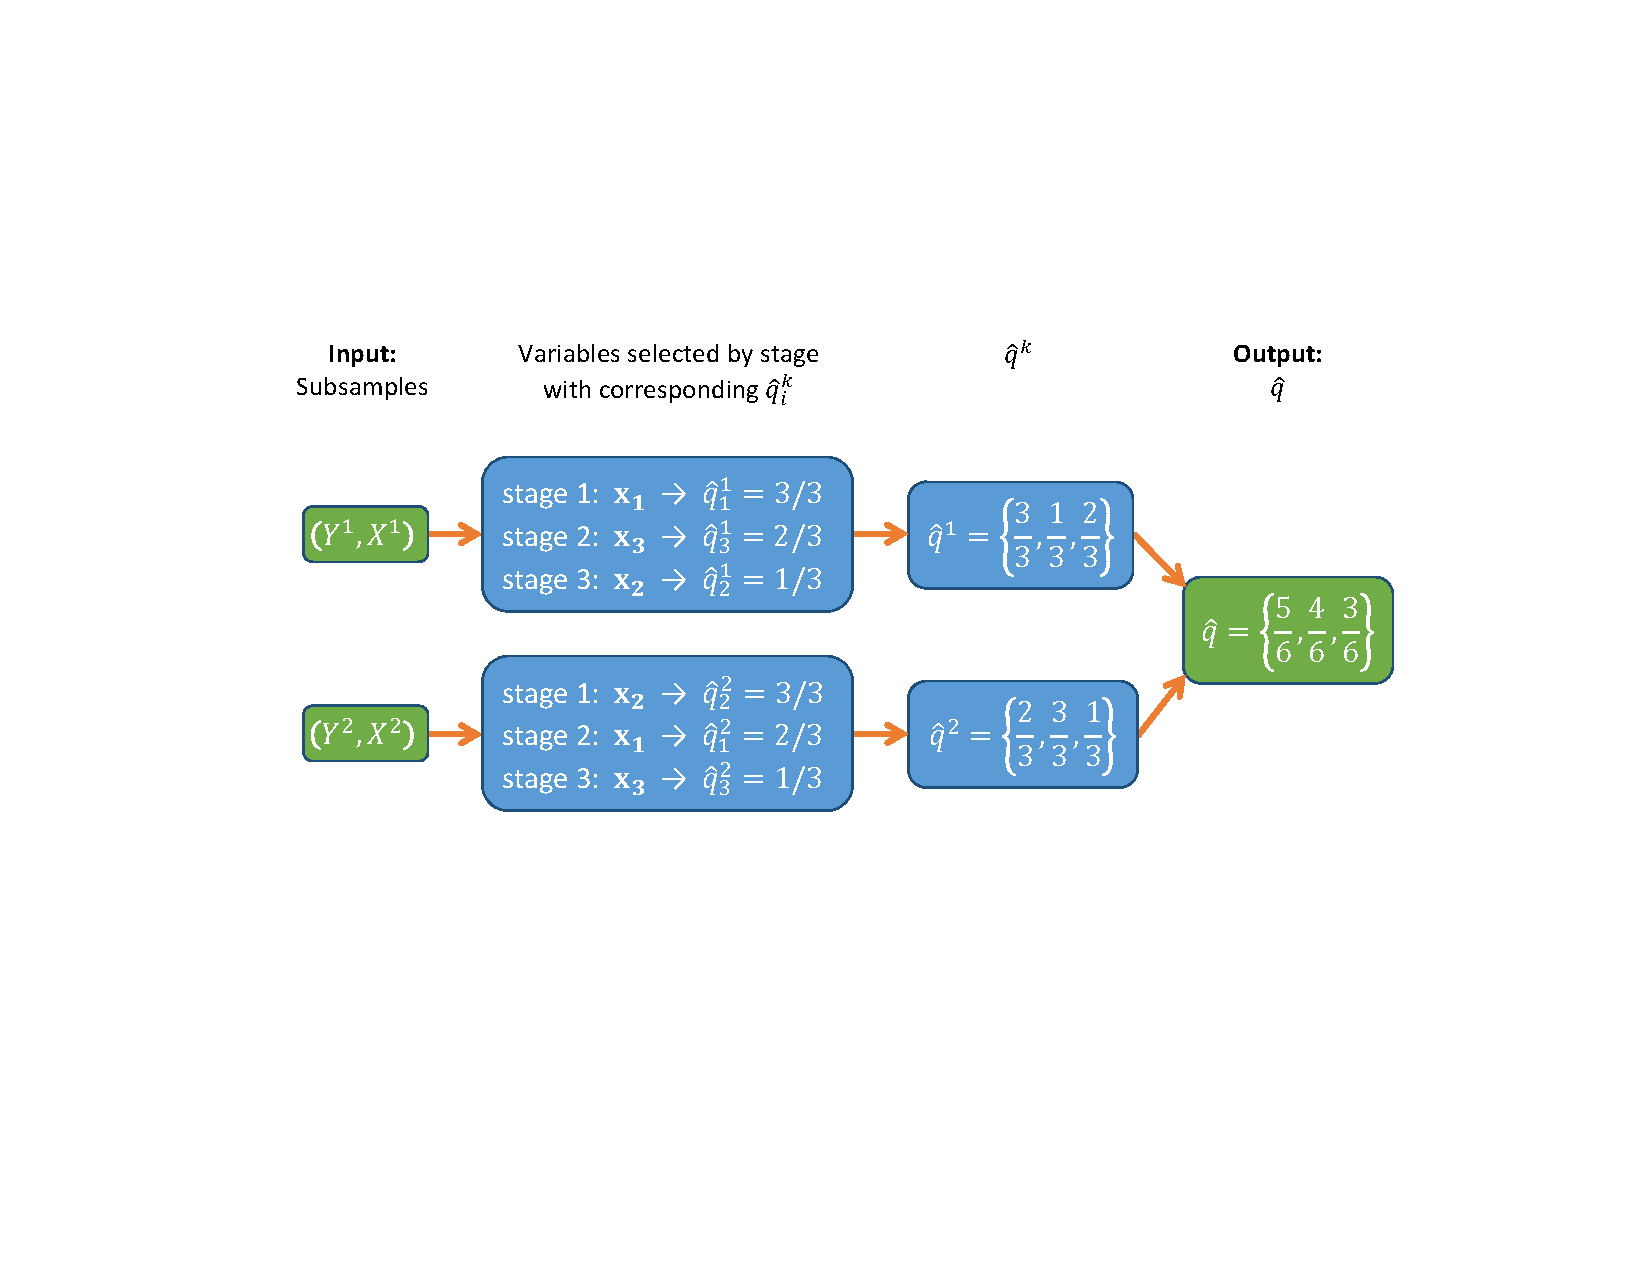
\includegraphics[width=0.95\paperwidth]{q_demo_1new.pdf}
    %
      \caption{Computation of $\widehat{q}$ on 2 subsamples, where $\left\{ \mathbf{x}_1, \mathbf{x}_2 \right\}$ are informative and $\mathbf{x}_3$ is redundant.}
    %
      \label{fig:q_demo}
    %
  \end{figure}
  %
\end{frame}

\begin{frame}{Theoretical properties of path averaging}
  %
  To justify theoretically the $\widehat{q}$ method, we use the \citet{zhang09} framework to derive the theoretical properties of path averaging (see Appendix~A).

  \begin{itemize}
    \item Under the \citet{zhang09} conditions, Lemma~A1 shows that, with a high probability, using $\widehat{q}^{\,k}_i$ ranking for variable selection on $\left( Y^k, X^k \right)$ generates the same theoretical results as the \citet{zhang09} forward selection method.
    %
    \item Under a similar stopping condition to \citet{zhang09}, Lemma~A2 shows that, with a high probability, there exists a threshold $c^k$ for the $L_0$ path on $\left( Y^k, X^k \right)$ such that $\widehat{q}^{\,k}_i \geqslant c^k$ for informative $\mathbf{x}_i$ and $\widehat{q}^k_i < c^k$ for redundant $\mathbf{x}_i$
    %
    \item Using Lemma~A2, Lemma~A3 shows that there exists a threshold $c = \sum_{i=k}^{K} c^k/K$ for the average $L_0$ path such that $\widehat{q}_i \geqslant c$ for informative $\mathbf{x}_i$ and $\widehat{q}_i < c$ for redundant $\mathbf{x}_i$ with large probability.
    %
  \end{itemize}
  %
\end{frame}

\subsection{Solar variable selection}

\begin{frame}{Variable selection on the average path}
  %
  \begin{algorithm}[H]

    \SetKwData{Left}{left}\SetKwData{This}{this}\SetKwData{Up}{up}
    \SetKwFunction{Union}{Union}\SetKwFunction{FindCompress}{FindCompress}
    \SetKwInOut{Input}{input}\SetKwInOut{Output}{output}
  
    \smallskip
    Randomly select 20\% of the sample points as the validation set; denote the remaining points as the training set\;
  
    Estimate $\widehat{q}$ using Algorithm~\ref{algo:APE-lar} on the training set and compute $Q(c) = \left\{ \mathbf{x}_j \; \vert \; \widehat{q}_j \geqslant c, \forall j\right\}$ for all $c \in \left\{ 1, 0.98, \ldots, 0.02, 0 \right\}.$
  
    Run an OLS regression of each $Q(c)$ on $Y$ using the training set and find $c^*$, the value of $c$ that minimizes the validation error\;
  
    Compute the OLS coefficients of $Q(c^*)$ on $Y$ using the whole sample.
  
    \caption{Subsample-ordered least-angle regression (solar)}
  \end{algorithm}
  %
\end{frame}

\begin{frame}{Theoretical properties of solar variable selection}
  %
  Using the \citet{zhang09} framework and Lemmas~A2 and~A3, we derive the following theoretical results for variable selection (see Appendix~A).

  \begin{itemize}
    %
    \item Theorem~A1 shows that solar variable selection is $L_0$ consistent under similar sparse eigenvalue and irrepresentable conditions used to prove lasso consistency.
    %
    \item Under similar assumptions to \citet{zhang09}, Lemmas~A4 and A5 show that the number of omitted informative $\mathbf{x}_i$ and the probability of selecting at least one redundant $\mathbf{x}_i$ are restricted by sample size, the sparse eigenvalue condition, and the stopping condition.
    %
  \end{itemize}
  %
\end{frame}

\subsection{Comparison and generaization}

\begin{frame}{The key difference between solar and lasso}
  %
  The key difference between solar and the lasso-type estimators, and the source of the advantages of solar, is solution path averaging.
  %
  \begin{itemize}
    %
    \item Lasso and solar both use the solution path for variable selection. The difference between solar and lasso is that solar averages the solution path. 
    
    \item Lasso and its variants focus on optimizing the shrinkage parameter $\lambda$ (via cross validation), ignoring concerns about the reliability of the lasso path in high dimensions. Optimizing $\lambda$ on an unreliable path renders variable selection difficult. 
    
    \item By contrast, solar prioritizes averaging the solution path, which not only averages out  path unreliability in high dimensions, but also ranks all the informative variables at the start of the average $L_0$ path (as shown in Lemma~A2 and~A3). 
    
    \item Hence, with a high probability, the variable selection algorithm needs only to analyze the variables at the start of the average $L_0$ path, making selection accurate and efficient.
    %
  \end{itemize}
  %
\end{frame}

\begin{frame}{The key difference between solar and bootstrap selection}
  %
  The difference between solar and lasso-related bootstrap selection (e.g., bolasso) is in how they average the variable selection algorithm.
  %
  \begin{itemize}
    %
    \item  Given the $\lambda$ value (optimal or not), lasso-related bootstrap selection averages the selection \emph{results} across subsamples. Thus, bootstrap selection requires hundreds of repetitions to average out the instability and redundancy of lasso variable selection \citep{bach2008bolasso}. 
    
    \item By contrast, solar averages solution \emph{paths}, which solves most of the lasso instability and redundancy issues, returning a more reliable average $L_0$ path. Variable selection along a reliable path substantially reduces the likelihood that solar selects redundant variables or omits informative variables. 
    
   \item As a result, solar-related bootstrap selection (e.g., bootstrap solar or solar stability selection) requires only 3-5 repetitions to outperform hundreds of lasso-related bootstrap repetitions (see Section~4.6 below for details).
  %
  \end{itemize}
  %
\end{frame}

\begin{frame}{Solar-cd and its generalization to lasso variants}
  
  \begin{algorithm}[H]

    \SetKwData{Left}{left}\SetKwData{This}{this}\SetKwData{Up}{up}
    \SetKwFunction{Union}{Union}\SetKwFunction{FindCompress}{FindCompress}
    \SetKwInOut{Input}{input}\SetKwInOut{Output}{output}
  
    \smallskip
    \Input{$\left( Y, X \right)$.}
  
    generate $K$ subsamples $\left\{ \left( Y^k, X^k \right) \right\}^{K}_{k=1}$ by randomly remove $1/K$ of observations in $\left( Y, X \right)$\;
  
    set $\widetilde{p} = \min\left\{ n_{\mathrm{sub}}, p \right\}$ \;
  
    \For{ k := 1 to K, stepsize = 1 \nllabel{outer_averaging_start3} }{
  
      denote $\lambda_s$ as the shrinkage parameter value that coordinate descent lasso selects $s$ variables, $\forall s \in \left[ 0, \widetilde{p}\right]$;
  
      run a pathwise coordinate descent for lasso on $\left( Y^k, X^k \right)$, $\forall \lambda \in \left\{\lambda_0, \lambda_1, \ldots, \lambda_{\widetilde{p}},\right\}$
  
      record the order of variable inclusion at each $\lambda \in \left\{\lambda_0, \lambda_1, \ldots, \lambda_{\widetilde{p}},\right\}$\;
  
      define $\widehat{q}^k = \mathbf{0} \in \mathbb{R}^p$\;
  
      $\forall i,s \in \mathbf{N}^+$, if $\mathbf{x}_i$ is included at $\lambda = \lambda_s$ and excluded at $\lambda_{s-1}$, set $\widehat{q}^k_i= (\widetilde{p} + 1 - s) / \widetilde{p}$, where $\widehat{q}^k_i$ is the $i$\textsuperscript{th} entry of $\widehat{q}^k$\;
  
    }
  
    $\widehat{q} := \frac{1}{K} \sum_{k=1}^{K} \widehat{q}^k$\; \nllabel{outer_averaging_end3}
  
    \Return $\widehat{q}$
  
  \caption{average $L_0$ solution path estimation via coordinate descent \label{algo:APE-cd}}
  
  \end{algorithm}

\end{frame}

\begin{frame}{Solar-cd and its generalization to lasso variants}

   Many lasso enhancements (e.g., safe/strong rules, post-lasso hypothesis testing) may be applied to solar because they use the same optimization methods. Because solar is trained by least angle regression or coordinate descent, it can easily be extended to several lasso variants

  \begin{itemize}
    %
    \item `Grouped solar' is invoked by forcing specific variables to be simultaneously selected into the solution path;
    %
    \item `Adaptive solar' is obtained by weighting variable rankings in the average $L_0$ path according to their OLS coefficients;
    %
    \item `Solar elastic net' or `fused solar' is derived by replacing the coordinate descent loss function in Algorithm~\ref{algo:APE-cd} with the $L_1$-$L_2$ loss
      %
      \begin{equation}
        %
        \left\Vert Y -X\beta \right\Vert_2^2 + \lambda^{(1)} \left\Vert \beta \right\Vert_1 + \lambda^{(2)} \left\Vert \beta \right\Vert_2^2
        %
      \end{equation}
      %
      or fused loss
      %
      \begin{equation}
        %
        \left\Vert Y -X\beta \right\Vert_2^2 + \lambda^{(1)} \left\Vert \beta \right\Vert_1 + \lambda^{(2)} \sum_{j=2}^{p} \left\vert \beta_j - \beta_{j-1} \right\vert_1.
        %
      \end{equation}
      %
  \end{itemize}

\end{frame}

%%%%%%%%%%%%%%%%%%%%%%%%%%%%%%%%%%%%%%%%%%%%%%%%%%%%%%%%%%%%%%%%%%%%%%
%%%%%%%%%%%%%%%%%%%%%%%%%%%%%%%%%%%%%%%%%%%%%%%%%%%%%%%%%%%%%%%%%%%%%%
%%%%%%%%%%%%%%%%%%%%%%%%%%%%%%%%%%%%%%%%%%%%%%%%%%%%%%%%%%%%%%%%%%%%%%

\section{Solar advantages over other methods}

\subsection{Post-selection hypothesis testing}

\begin{frame}{Post-selection hypothesis testing}
  %
  \begin{itemize}
    %
    \item Because the lasso tests \citep{lockhartall14, taylor2014exact} are based on forward regression, they may be adapted to solar;
    %
    \item A major advantage of solar is its amenability to post-selection testing. More interestingly, by replacing lasso with solar for the post-selection tests (e.g, the data-splitting tests) \citep{wasserman2009high,meinshausen2009p}, we can substantially improve the testing accuracy for weak signal detection under limited $n$;
    %
  \end{itemize}
  %
\end{frame}

\begin{frame}{Example 1}
  %
  Consider the DGP
  %
  \begin{equation}
    Y = \mathbf{x}_0 + 2 \mathbf{x}_1 + 3 \mathbf{x}_2 + 4 \mathbf{x}_3 + 5 \mathbf{x}_4 + \sum_{j=5}^{p} 0 \cdot \mathbf{x}_j + e,
  \end{equation}
  %
  where $\mathbf{x}_i$, $i=0,\dots,p$, are standard Gaussian variables with pairwise correlations of $0.5$, $e$ is a standard Gaussian noise term, and $p/n=140/120$.
  
  We conduct a data-splitting test \citep{romano2019multiple,diciccio2020exact} by randomly separating the data into two portions of 60 observations. In the first round, one portion is used for solar or lasso selection and the other for testing. In the second round, the roles of the two portions are reversed. We may apply Theorem~3.2 of \citet{romano2019multiple} and compute the average p-value across the two rounds to conduct a valid t-test for any selected covariate.
  %
\end{frame}

\begin{frame}{Example 1}
  %
  \begin{figure}[ht]
    %
      \centering
    %
      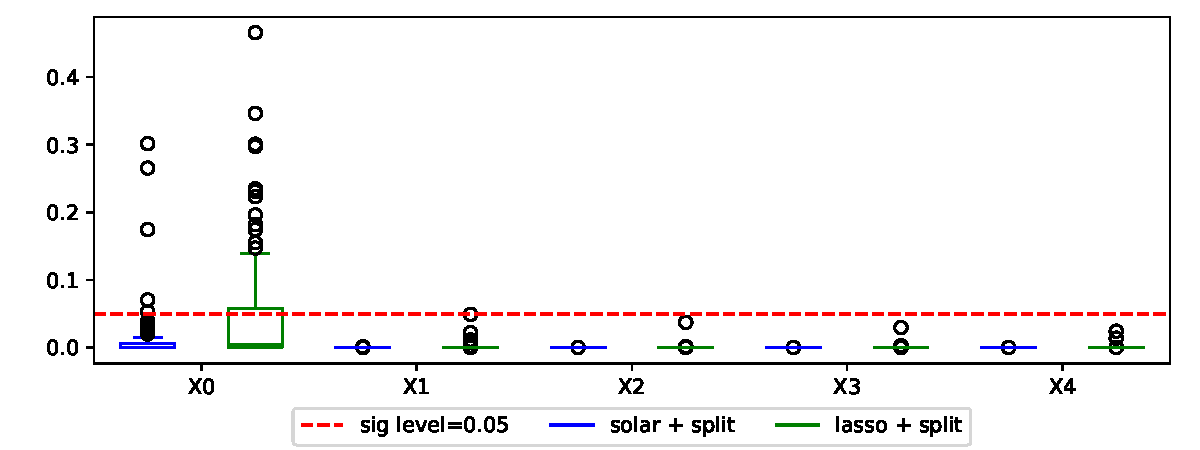
\includegraphics[width=0.9\paperwidth]{p_value_compare.pdf}
    %
      \caption{Average p-value boxplots for data-splitting t-tests with solar and lasso.}
    %
      \label{fig:p_value_compare}
    %
  \end{figure}
  %
  solar p-values are more reliable for detecting weak signals with limited $n$ and large $p$
\end{frame}

\subsection{Variable selection under complicated dependence structures}

\begin{frame}{informative variables are unconditionally uncorrelated to $Y$}
  %
  \begin{figure}[ht]
    %
    \centering
    %
    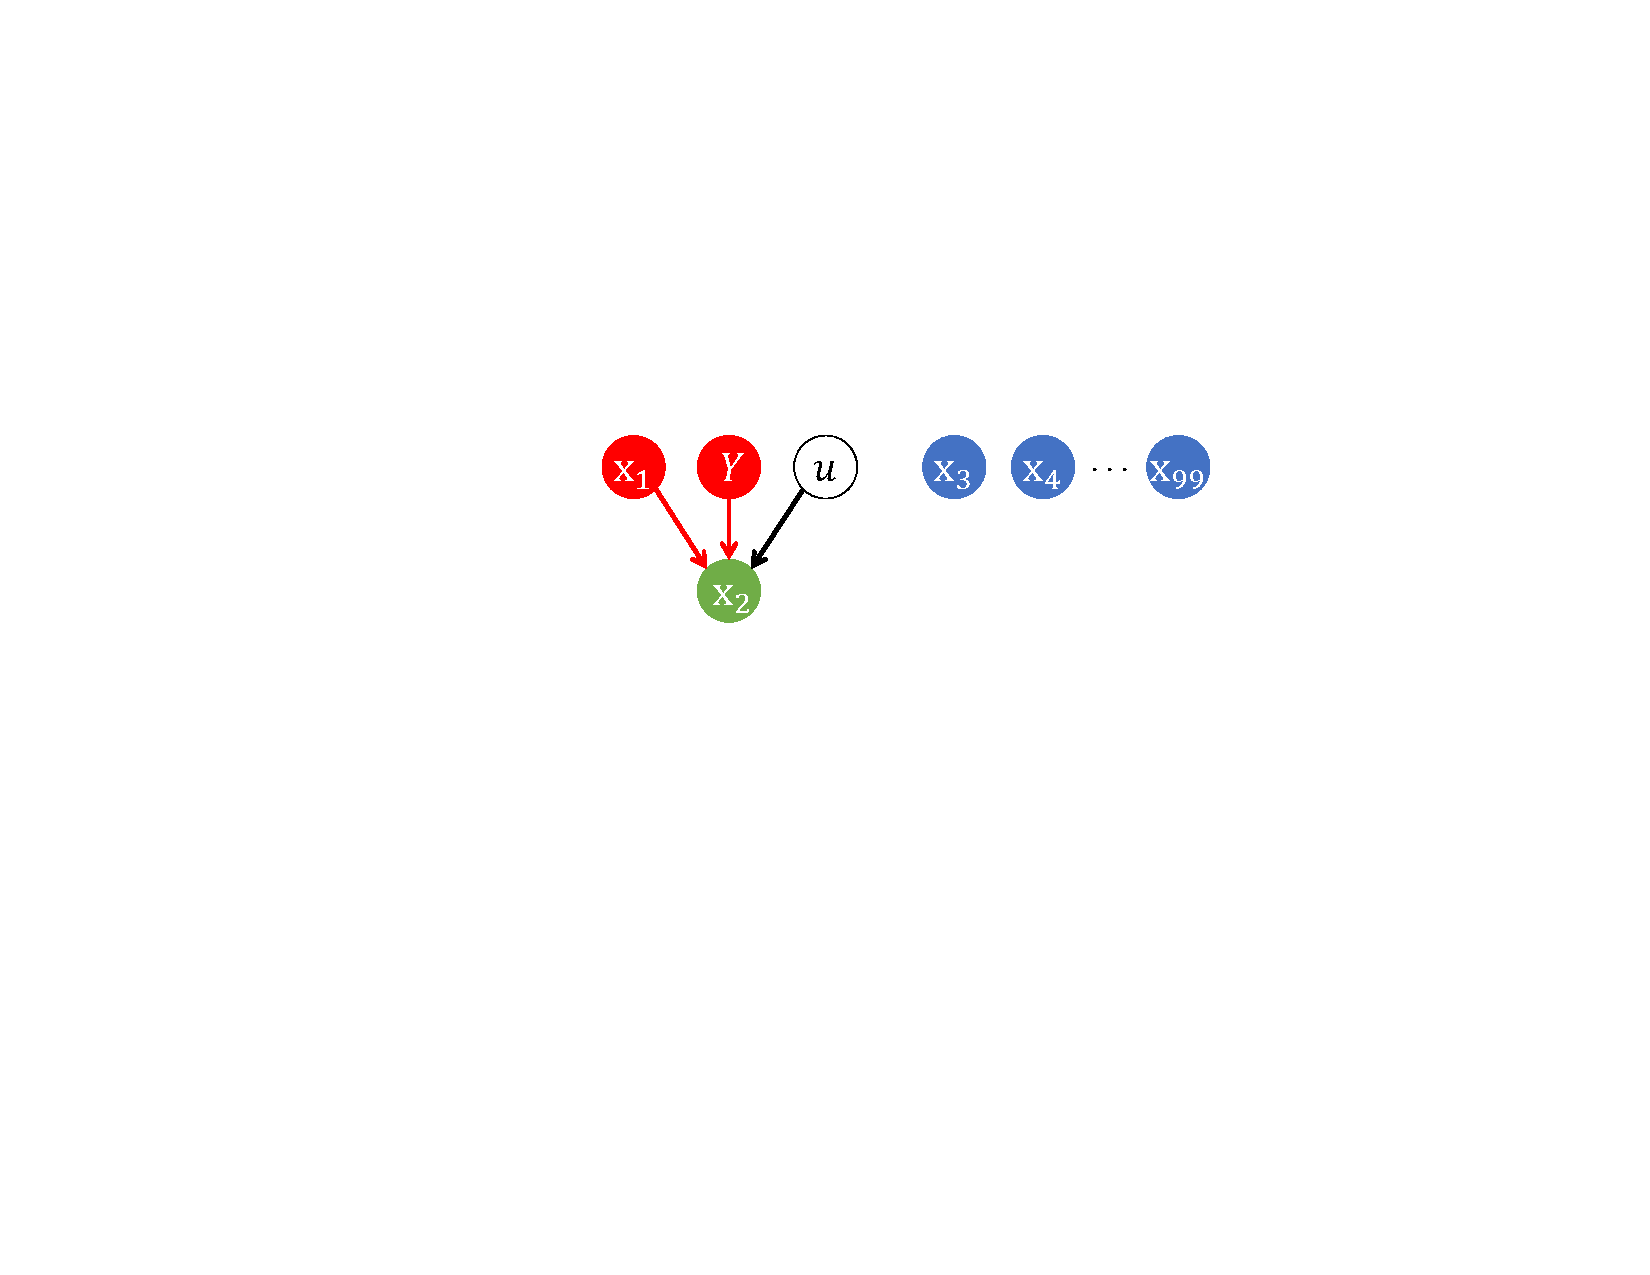
\includegraphics[width=0.6\paperwidth]{uncond_example.pdf}
    %
    \caption{Y is unconditionally uncorrelated with an informative $\mathbf{x}_1$.}
    %
    \label{fig:uncond_example}
    %
  \end{figure}
  %
  In Figure~\ref{fig:uncond_example}, there are $100$ variables and $\mathbf{x}_2$ is (causally) generated by its parents $\left\{ \mathbf{x}_1, Y \right\}$ as follows,
  %
  \begin{equation}
    %
    \mathbf{x}_2 = \alpha_1 \mathbf{x}_1 + \alpha_2 Y + u,
    %
    \label{eqn:collider_1}
    %
  \end{equation}
  %
  where $\mathbf{x}_1$ is unconditionally uncorrelated with $Y$, $\mathbf{x}_1$ and $Y$ are both unconditionally and conditionally uncorrelated with the redundant variables $\{\mathbf{x}_3, \ldots, \mathbf{x}_{99}\}$, $\left\{\alpha_1, \alpha_2 \right\}$ are population regression coefficients, and $u$ is a Gaussian noise term.
  %
\end{frame}

\begin{frame}{Example 2a}
   If $Y$ is chosen to be the response variable, the population regression equation is
  %
  \begin{equation}
    %
    Y = -\frac{\alpha_1}{\alpha_2} \mathbf{x}_1 + \frac{1}{\alpha_2} \mathbf{x}_2 - \frac{1}{\alpha_2}u.
    %
    \label{eqn:collider_2}
    %
  \end{equation}
  %
  Note that $\mathbf{x}_1$ and $\mathbf{x}_2$ are both informative for $Y$. However, since $\mathbf{x}_1$ is unconditionally uncorrelated with $Y$ in the population.
  %
\end{frame}

\begin{frame}{Example 2a}

  For a given value of the shrinkage parameter $\lambda$ in grid search, the base strong rule and the safe rule for lasso to reject a selected variable, respectively, satisfies (\ref{eqn:safe_rule}) and (\ref{eqn:strong_rule}):
  %
  \begin{eqnarray}
    %
    \left\vert \mathbf{x}_1^T Y \right\vert < & \lambda - \left\Vert \mathbf{x}_i \right\Vert_2 \left\Vert Y \right\Vert_2 \frac{\lambda_{max} - \lambda} {\lambda_{max}} ; \label{eqn:safe_rule} \\
    %
    \left\vert \mathbf{x}_1^T Y \right\vert < & 2\lambda - \lambda_{max} , \label{eqn:strong_rule}
    %
    \label{eqn:post_estmation_rule}
    %
  \end{eqnarray}
  %
  where the $\mathbf{x}_i$ are standardized and $\lambda_{max}$ is the value of the shrinkage parameter that rejects all the variables. Both rules are based on the unconditional covariance between $\mathbf{x}_1$ and $Y$, which is $0$ in population.

\end{frame}

\begin{frame}{redundant variables are unconditionally correlated to $Y$}
  %
  \begin{figure}[ht]
    %
    \centering
    %
    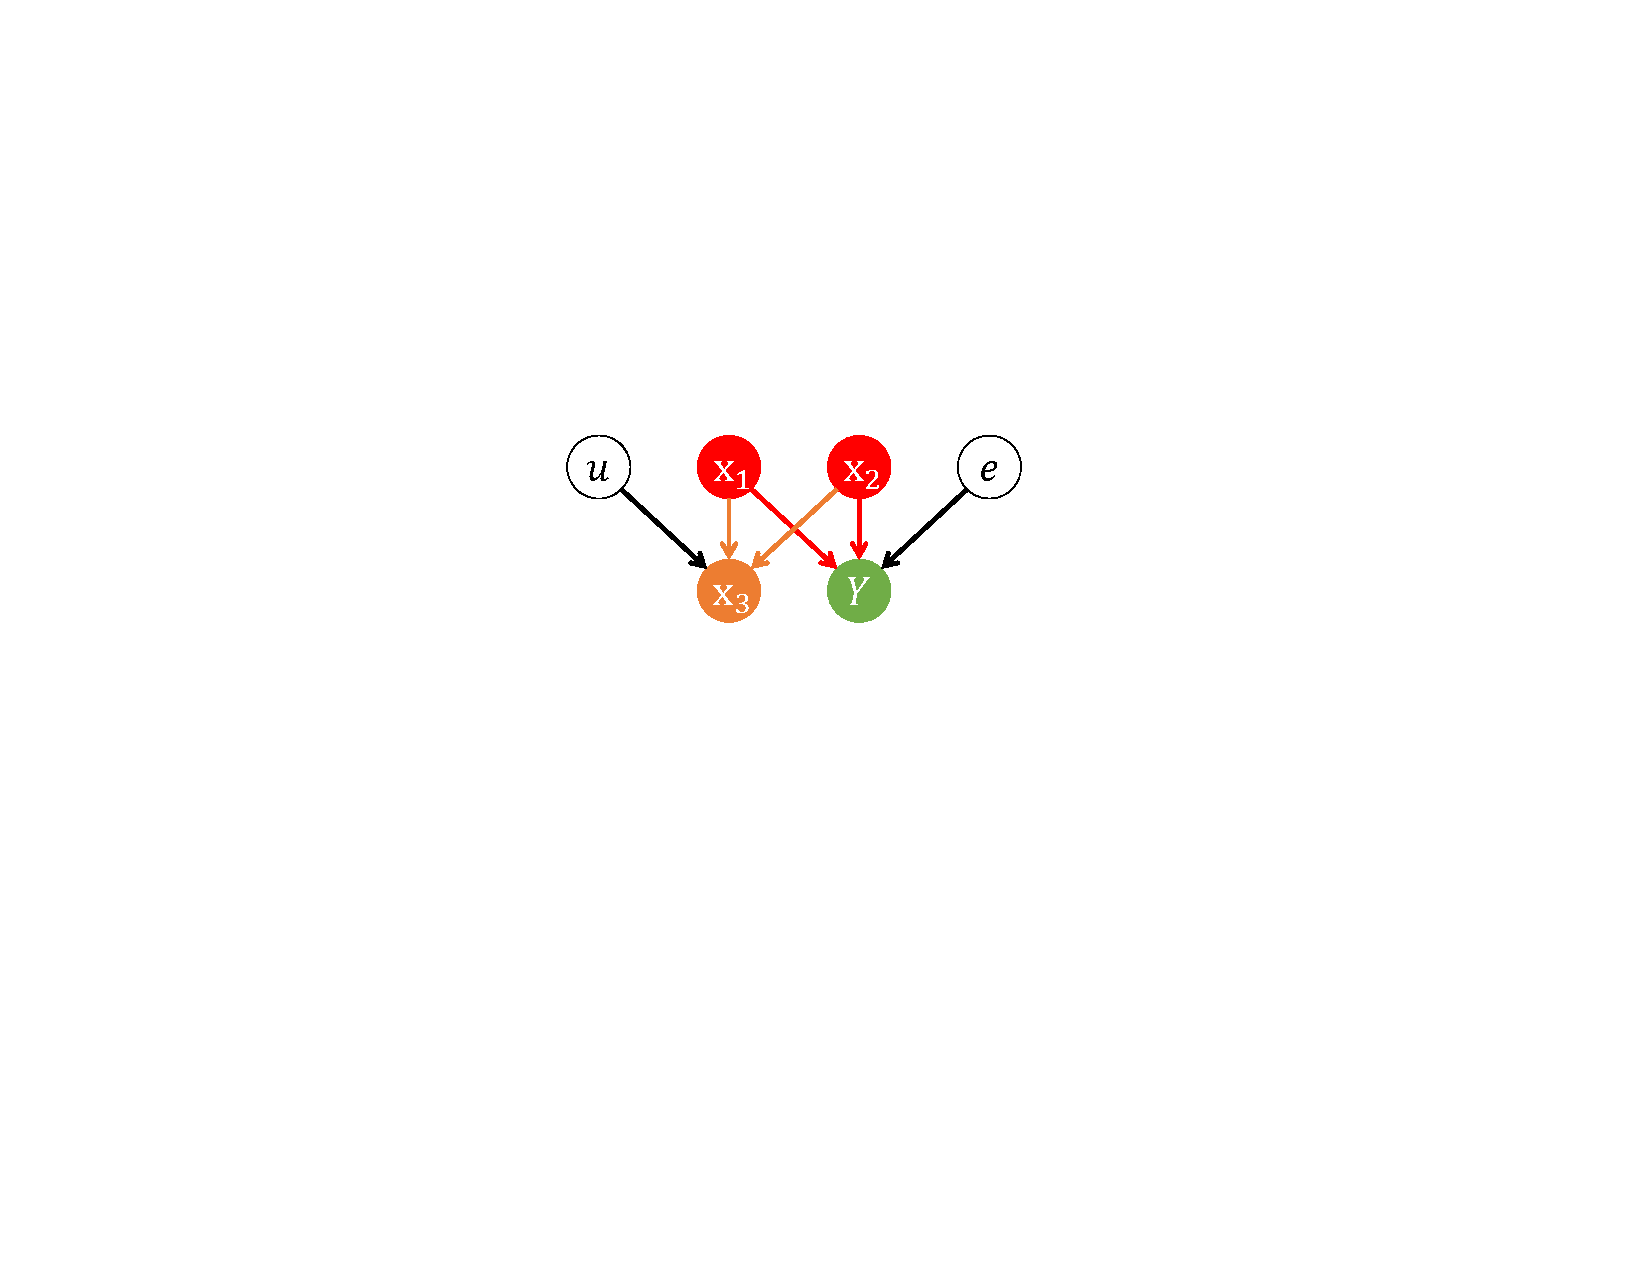
\includegraphics[width=0.35\paperwidth]{example3.pdf}
    %
    \caption{$Y$ is unconditionally correlated with a redundant $\mathbf{x}_3$.}
    %
    \label{fig:cond_example}
    %
  \end{figure}
  %
  
  Figure~\ref{fig:cond_example} depicts the following confounding structure,
  %
  \begin{equation}
    %
    \begin{cases}
    %
      \mathbf{x}_3 = \frac{1}{3} \mathbf{x}_1 + \frac{1}{3} \mathbf{x}_2 + \frac{\sqrt{7}}{3} u, \\
      %
      Y = \frac{7}{10} \mathbf{x}_1 +  \frac{2}{10} \mathbf{x}_2 +  \frac{\sqrt{47}}{10} e, \\
      %
    \end{cases}
    %
    \label{eqn:example_4}
    %
  \end{equation}
  %
  where $\mathbf{x}_1$ and $\mathbf{x}_2$ cause both $Y$ and $\mathbf{x}_3$, implying that $\mathbf{x}_3$ is unconditionally correlated to $Y$; $\mathbf{x}_1$, $\mathbf{x}_2$, $u$ and $e$ are independent; $\mathbf{x}_3$ is independent from $e$; $Y$ is independent from $u$; and all variables are standardized.
\end{frame}

\begin{frame}{Example 2b}
  
  For large $n$, when the sample correlations are close to their population values, the sample marginal correlations to $Y$ are:
  %
  \begin{equation}
    %
    \begin{aligned}
      %
      \mathrm{corr} \left( \mathbf{x}_1, Y \right)  = & \;0.7, \\
      %
      \mathrm{corr} \left( \mathbf{x}_3, Y \right)  = & \;\mathrm{corr} \left( \frac{1}{3} \mathbf{x}_1 + \frac{1}{3} \mathbf{x}_2, \frac{7}{10} \mathbf{x}_1 +  \frac{2}{10} \mathbf{x}_2 \right)
      %
      = 0.3, \\
      %
      \mathrm{corr} \left( \mathbf{x}_2, Y \right)  = & \;0.2. \\
      %
    \end{aligned}
    %
  \end{equation}
  %
  Because $\mathbf{x}_2$ ranks below $\mathbf{x}_1$ and $\mathbf{x}_3$ in terms of marginal correlations to $Y$, the variable screening method must select all $3$ variables---including the redundant $\mathbf{x}_3$---to avoid omitting $\mathbf{x}_2$. The base strong rule and safe rule may also have difficulty rejecting $\mathbf{x}_3$. Since $\mathrm{corr} \left( \mathbf{x}_3, Y \right)>\mathrm{corr} \left( \mathbf{x}_2, Y \right)$, if lasso selects $\mathbf{x}_3$ and $\mathbf{x}_2$ and the strong (or safe) rule is used to reject $\mathbf{x}_3$, $\mathbf{x}_2$ will also be rejected.
\end{frame}

\begin{frame}{Example 2b}

  Forward regression, solar, and lasso will not make the same error. In forward regression, $\mathbf{x}_1$ will be included at the first stage. After controlling for $\mathbf{x}_1$, the partial correlations (for large $n$) of both $\mathbf{x}_2$ and $\mathbf{x}_3$ with $Y$ are:
  %
  \begin{equation}
    %
    \begin{aligned}
      %
      \mathrm{corr} \left( \mathbf{x}_2, Y \vert \mathbf{x}_1 \right)  = & \;\mathrm{corr} \left( \mathbf{x}_2, \frac{2}{10} \mathbf{x}_2 \right)
      %
      = 0.2, \\
      %
      \mathrm{corr} \left( \mathbf{x}_3, Y \vert \mathbf{x}_1 \right)  = & \;\mathrm{corr} \left( \frac{1}{3} \mathbf{x}_1 + \frac{1}{3} \mathbf{x}_2, \frac{2}{10} \mathbf{x}_2 \right)
      %
      = 0.0667. \\
      %
    \end{aligned}
    %
  \end{equation}
  %
  Because $\mathrm{corr}(\mathbf{x}_2, Y \vert \mathbf{x}_1)>\mathrm{corr}(\mathbf{x}_3, Y \vert \mathbf{x}_1)$, forward regression will include $\mathbf{x}_2$, not $\mathbf{x}_3$, at the second stage. After controlling for $\mathbf{x}_1$ and $\mathbf{x}_2$, remaining variation in $Y$ is due to $e$, which $\mathbf{x}_3$ cannot explain. Thus, CV or BIC will terminate forward regression after the second stage and $\mathbf{x}_3$ will not be selected. Similarly, because solar relies on the average $L_0$ path, it will include $\mathbf{x}_1$ and $\mathbf{x}_2$ but not $\mathbf{x}_3$.

\end{frame}

\begin{frame}{Robustness to IRC}

  \begin{definition}[IRC]
    Given $F \subset \left\{ 1, \ldots, p \right\}$, define $X_F$ to be the $n \times \left\vert F \right \vert$ matrix with only the full set of informative variables. Define
    %
      \begin{align}
      %
      \mu \left( F \right) = & \max \left\{ \left\Vert \left( \left( X_F \right)^T X_F \right)^{-1} \left( X_F \right)^T \mathbf{x}_j \right\Vert_1 \; \vert \; \forall j \not\in F \right\}. \notag
      %
      \end{align}
    %
    Given a constant $0 < \eta \leqslant 1$, the \emph{strong} irrepresentable condition is satisfied if $\mu \left( F \right) \leqslant 1 - \eta$ and the \emph{weak} irrepresentable condition is satisfied if $\mu \left( F \right) < 1$.$\blacksquare$
  \end{definition}
\end{frame}

\begin{frame}{Example 3}  
  
  Modify the DGP in Example~2b to match the \citet{zhaoyu06} simulations. Thus, $n = 200$, $p = 50$, and $\{\mathbf{x}_0, \ldots, \mathbf{x}_4, \mathbf{x}_6, \ldots, \mathbf{x}_{50}\}$ are generated from a zero-mean, unit-variance multivariate Gaussian distribution, where all the correlation coefficients are $0.5$. The DGP of $Y$ and $\mathbf{x}_5$ is
  \begin{equation}
    %
    \begin{cases}
    %
      \mathbf{x}_5 = \omega \mathbf{x}_0 + \omega \mathbf{x}_1 + \gamma\cdot \sqrt{1 - 2\omega^2} \\
      %
      Y = 2 \mathbf{x}_0 + 3\mathbf{x}_1 + 4 \mathbf{x}_2 + 5 \mathbf{x}_3 + 6 \mathbf{x}_4 + e \\
      %
    \end{cases}
    %
    \label{eqn:dgp_x5}
    %
  \end{equation}
  %
  where $\omega \in \mathbb{R}$, while $\gamma$ and $e$ are both standard Gaussian noise terms, independent from one another and all the other variables. Compared with Example~2b, this DGP increases the challenge of accurate selection by increasing the number of redundant variables from 1 to 46, $\{\mathbf{x}_5, \ldots, \mathbf{x}_{50}\}$. This DGP also makes it straightforward to control the IRC through $\omega$, which affects the value of $\mu \left( F \right)$.

\end{frame}

\begin{frame}{Example 3}  

  \begin{figure}
    %
    \centering
    %
    \subfloat[\label{fig:solar_ic_type-II1}$\omega = 1/4,\;\mu\left(F\right)=1/2$, lasso]
    {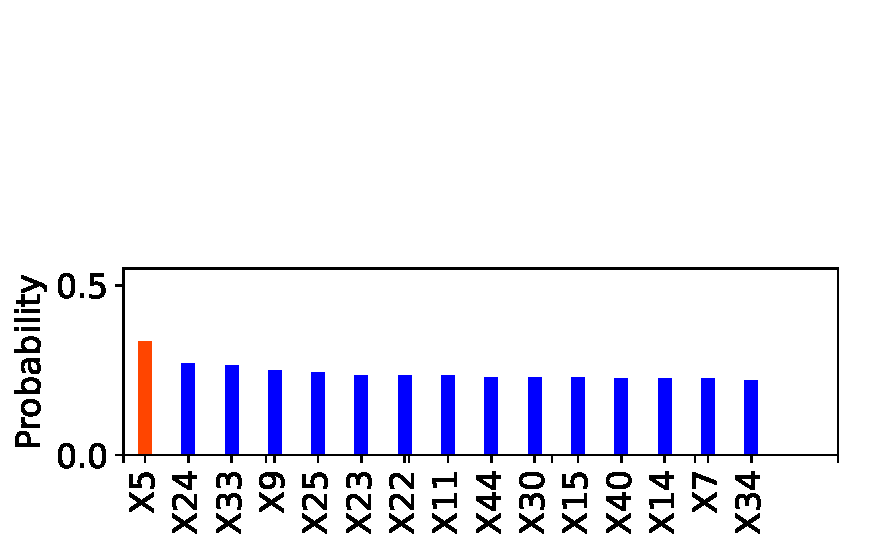
\includegraphics[width=0.32\paperwidth]{acc_plot_top20_ic_25_False_lars-crop.pdf}}
    %
    \subfloat[\label{fig:solar_ic_type-II2}$\omega = 1/3,\;\mu\left(F\right)=2/3$, lasso]
    {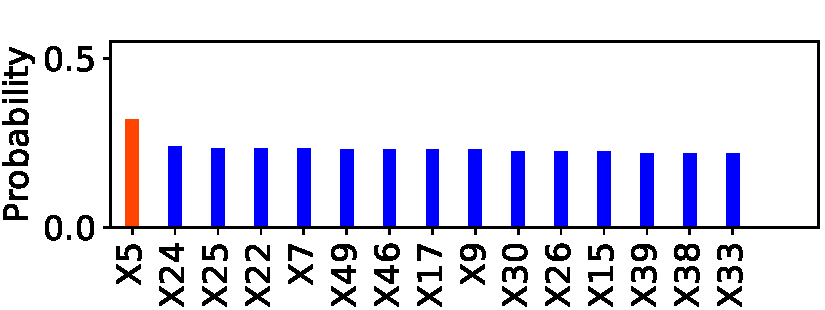
\includegraphics[width=0.32\paperwidth]{acc_plot_top20_ic_33_False_lars-crop.pdf}}
    %
    \subfloat[\label{fig:solar_ic_type-II3}$\omega = 1/2,\;\mu\left(F\right)=1$, lasso]
    {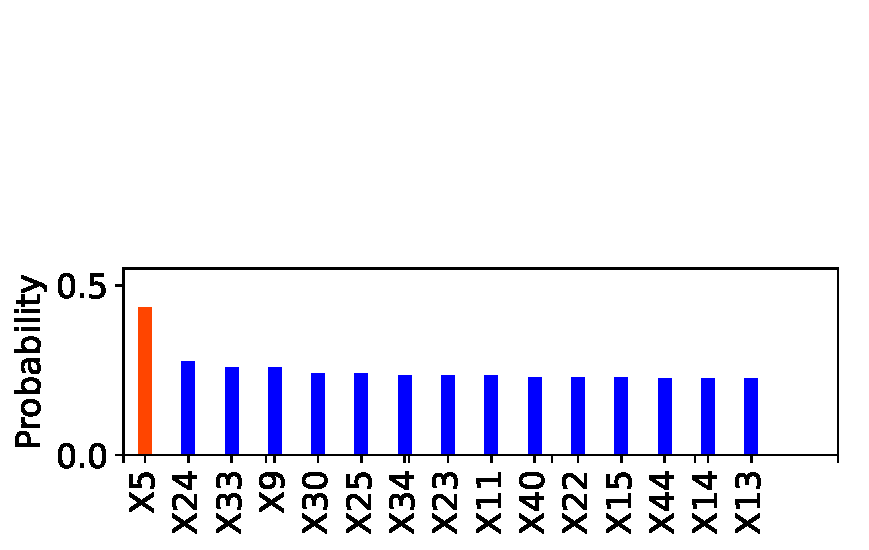
\includegraphics[width=0.32\paperwidth]{acc_plot_top20_ic_5_False_lars-crop.pdf}}

    \subfloat[\label{fig:solar_ic_type-II7}$\omega = 1/4,\;\mu\left(F\right)=1/2$, solar]
    {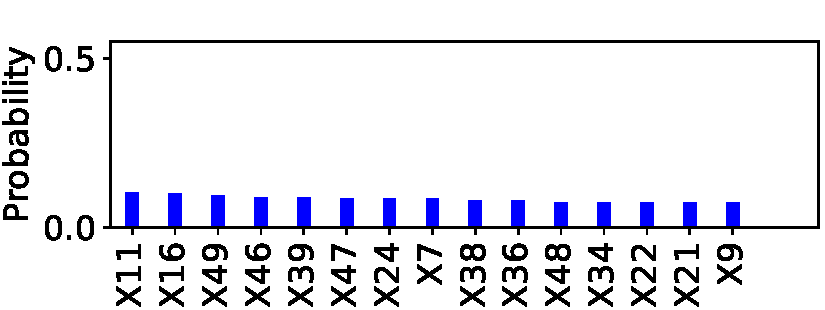
\includegraphics[width=0.32\paperwidth]{acc_plot_top20_ic_25_False_solar-crop.pdf}}
    %
    \subfloat[\label{fig:solar_ic_type-II8}$\omega = 1/3,\;\mu\left(F\right)=2/3$, solar]
    {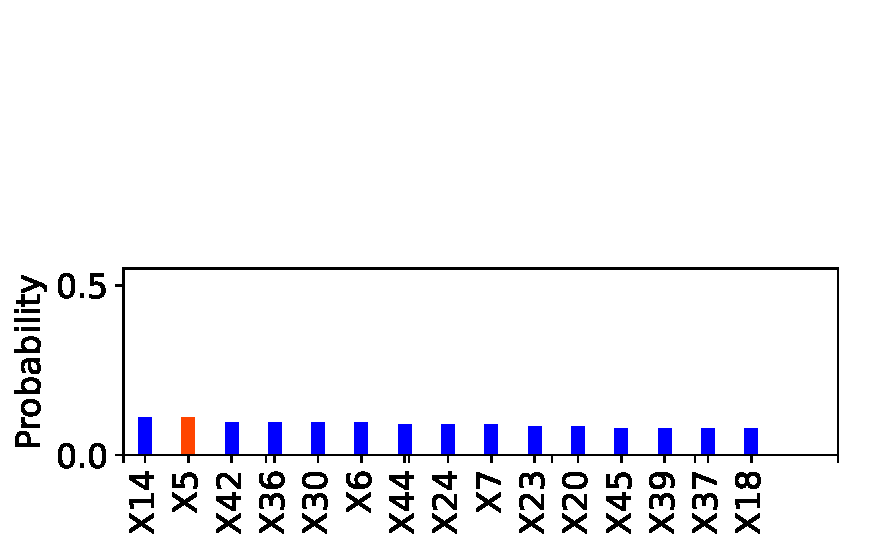
\includegraphics[width=0.32\paperwidth]{acc_plot_top20_ic_33_False_solar-crop.pdf}}
    %
    \subfloat[\label{fig:solar_ic_type-II9}$\omega = 1/2,\;\mu\left(F\right)=1$, solar]
    {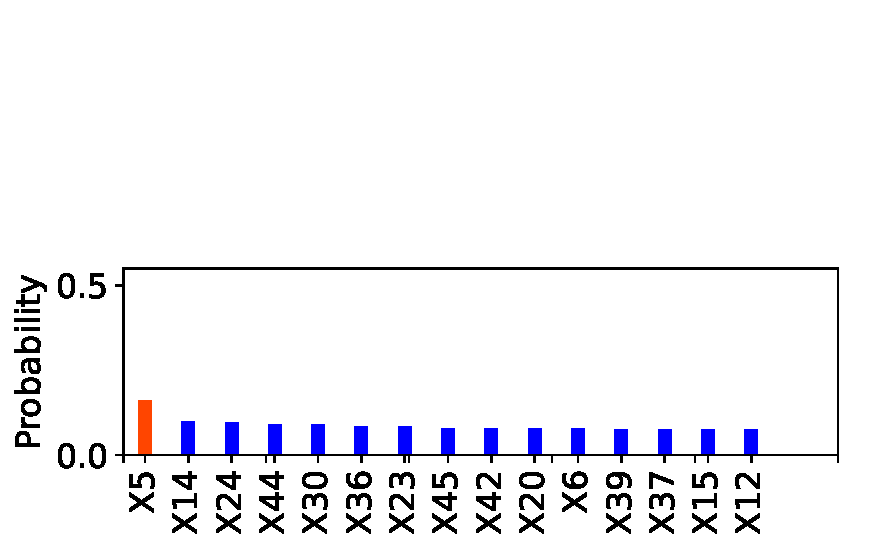
\includegraphics[width=0.32\paperwidth]{acc_plot_top20_ic_5_False_solar-crop.pdf}}
    %
    \caption{Probability of including redundant variables (top 15) in simulation~2 ($\mathbf{x}_5$ in orange).}
    \label{fig:solar_ic_type-II}
    %
  \end{figure}

\end{frame}

%%%%%%%%%%%%%%%%%%%%%%%%%%%%%%%%%%%%%%%%%%%%%%%%%%%%%%%%%%%%%%%%%%%%%%%%%%%%%%
%%%%%%%%%%%%%%%%%%%%%%%%%%%%%%%%%%%%%%%%%%%%%%%%%%%%%%%%%%%%%%%%%%%%%%%%%%%%%%
%%%%%%%%%%%%%%%%%%%%%%%%%%%%%%%%%%%%%%%%%%%%%%%%%%%%%%%%%%%%%%%%%%%%%%%%%%%%%%

\section{Solar advantages over lasso and bootstrap selection}

\begin{frame}{Simulation DGP}
  
  The DGP for the simulations is as follows. The $p$ covariates in $X \in \mathbb{R}^{n \times p}$ are generated from a zero-mean, multivariate Gaussian distribution, with all off-diagonal elements in the covariance matrix equal to~0.5. The first 5 variables in $X$ are informative; the remaining $p-5$ variables are redundant. The response variable $Y \in \mathbb{R}^{n \times 1}$ is:
  %
  \begin{equation}
  %
    Y =  2 \mathbf{x}_0 + 3 \mathbf{x}_1 + 4 \mathbf{x}_2 + 5 \mathbf{x}_3 + 6 \mathbf{x}_4  + e,
    \label{eqn:pop_model}
  \end{equation}
  %
  where $e\in \mathbb{R}^{n \times 1}$ is a standard Gaussian noise term. All data points are independently and identically distributed. Each $\mathbf{x}_i$, $i=1,\ldots,p$, is independent from the noise term $e$, which is standard Gaussian. Simulations are repeated 200 times with fixed Python random generators across simulations.

\end{frame}

\subsection{Sparisty and accuracy comparison}

\begin{frame}{Sparisty and accuracy comparison}
  \begin{table}[H]
    %
    \centering
    %
    \caption{Simulation results for sparsity and accuracy.\label{table:sim_1}}
    %
    \resizebox{0.98\textwidth}{!}{%
    \renewcommand{\arraystretch}{0.9}
    \begin{tabular}{l ... ... ...}
      \toprule
      & \multicolumn{3}{c}{$p/n\rightarrow0$}
      & \multicolumn{3}{c}{$p/n\rightarrow1$}
      & \multicolumn{3}{c}{$\log(p)/n\rightarrow0$} \\
      \cmidrule(lr){2-4} \cmidrule(lr){5-7} \cmidrule(lr){8-10}
      & \multicolumn{1}{c}{$\frac{100}{100}$} & \multicolumn{1}{c}{$\frac{100}{150}$} & \multicolumn{1}{c}{$\frac{100}{200}$}
      & \multicolumn{1}{c}{$\frac{150}{100}$} & \multicolumn{1}{c}{$\frac{200}{150}$} & \multicolumn{1}{c}{$\frac{250}{200}$}
      & \multicolumn{1}{c}{$\frac{400}{200}$} & \multicolumn{1}{c}{$\frac{800}{400}$} & \multicolumn{1}{c}{$\frac{1200}{600}$}  \\
      \midrule
      \multicolumn{9}{l}{\emph{mean number of selected variables}}\\
      \hspace*{5mm}lasso        & 20.4 & 19.5 & 19.7 & 23.1 & 24.1 & 27.2 & 30.7 & 36.7 & 37.4 \\
      \hspace*{5mm}solar        & 10.5 &  9.3 &  9.1 & 10.7 &  9.8 &  8.7 & 11.4 & 16.1 & 18.5 \\
      \\ [-8pt]
      \hspace*{5mm}bolasso-S    &  5.5 &  6.4 &  6.5 &  5.5 &  6.4 &  6.5 &  5.7 &  6.6 &  7.6 \\
      \hspace*{5mm}bolasso-H    &  5   &  5   &  5   &  5   &  5   &  5   &  5   &  5   &  5   \\
      \\ [-8pt]
      \hspace*{5mm}bsolar-3S/3H &  5.4 &  5.2 &  5.1 &  5.4 &  5.2 &  5.1 &  5.3 &  5.8 &  6   \\
      \hspace*{5mm}bsolar-5S/5H &  5.2 &  5.1 &  5   &  5.2 &  5.1 &  5   &  5.1 &  5.2 &  5.4 \\
      \hspace*{5mm}bsolar-10S   &  5.2 &  5.1 &  5   &  5.2 &  5.1 &  5   &  5.1 &  5.2 &  5.3 \\
      \hspace*{5mm}bsolar-10H   &  5   &  5   &  5   &  5   &  5   &  5   &  5   &  5   &  5.1 \\
      \\ [-8pt] \multicolumn{9}{l}{\emph{mean number of selected informative variables}}\\
      \hspace*{5mm}lasso        &  5   &  5   &  5   &  5   &  5   &  5   &  5   &  5   &  5   \\
      \hspace*{5mm}solar        &  5   &  5   &  5   &  5   &  5   &  5   &  5   &  5   &  5   \\
      \hspace*{5mm}bolasso-S/H  &  5   &  5   &  5   &  5   &  5   &  5   &  5   &  5   &  5   \\
      \hspace*{5mm}bsolar-3S/3H/5S/5H/10S/10H & 5 & 5 & 5 & 5 & 5 & 5 & 5 & 5 & 5 \\
      \bottomrule
      \end{tabular}}
      %
    \end{table}
    
\end{frame}

\begin{frame}{Sparisty and accuracy comparison}

Table above also reveals several advantages of solar over lasso in bootstrap selection.
%
\begin{itemize}
  %
  \item In terms of variable selection, bolasso-S stands out with the poorest sparsity; the others perform almost identically.
  %
  \item Solar imposes less than $1/3$ of the lasso computation load, implying that bsolar-3 has the same computation load as lasso. Given bolasso requires 256 subsample lasso repetitions while bsolar-3 has the same computation load as one lasso realization, bsolar reduces subsample repetitions by 99\% relative to bolasso.
  %
  \item Bsolar, bolasso-H, and stability selection ($f>0.9$) return very similar sparsity and accuracy (on average selecting all the informative variables while rarely including a redundant variable). Based on the time complexity analysis of \citet{meinshausen2010stability}, bsolar-3 produces a reduction of at least $67$-$82\%$ in computation load relative to lasso stability selection.
  %
\end{itemize}

\end{frame}


\subsection{Subsample selection frequency comparison}

\begin{frame}{Subsample selection frequency comparison}

  \begin{table}[!htb]
    \caption{Subsample variable selection frequencies for bolasso and bsolar.}
    \label{table:subsample_select_freq}
    \begin{minipage}[t]{.55\linewidth}
      \small
      \subfloat[bolasso]{%
      \label{table:subsample_select_freq_1}
        \renewcommand{\arraystretch}{0.7}
        \begin{tabular}{cl}
          \toprule
          frequency & variables \\
          \midrule
          $\geqslant 1.00$ & $\mathbf{x}_4, \mathbf{x}_3, \mathbf{x}_2, \mathbf{x}_1, \mathbf{x}_0$ \\
          $\geqslant 0.88$ & $\mathbf{x}_4, \mathbf{x}_3, \mathbf{x}_2, \mathbf{x}_1, \mathbf{x}_0, \mathbf{x}_{28}$ \\
          $\geqslant 0.84$ & $\mathbf{x}_4, \mathbf{x}_3, \mathbf{x}_2, \mathbf{x}_1, \mathbf{x}_0, \mathbf{x}_{28}, \mathbf{x}_{71}$\\
          $\geqslant 0.76$ & $\mathbf{x}_4, \mathbf{x}_3, \mathbf{x}_2, \mathbf{x}_1, \mathbf{x}_0, \mathbf{x}_{28}, \mathbf{x}_{71}, \mathbf{x}_{91}$\\
          $\geqslant 0.70$ & $\mathbf{x}_4, \mathbf{x}_3, \mathbf{x}_2, \mathbf{x}_1, \mathbf{x}_0, \mathbf{x}_{28}, \mathbf{x}_{71}, \mathbf{x}_{91}, \mathbf{x}_{94}$\\
          $\geqslant 0.69$ & $\mathbf{x}_4, \mathbf{x}_3, \mathbf{x}_2, \mathbf{x}_1, \mathbf{x}_0, \mathbf{x}_{28}, \mathbf{x}_{71}, \mathbf{x}_{91}, \mathbf{x}_{94}, \mathbf{x}_{70}, \mathbf{x}_{40}$ \\
          $\vdots$ & $\vdots$ \\
          \bottomrule
      \end{tabular}}
    \end{minipage}
    \begin{minipage}[t]{.5\linewidth}
      \small
      \subfloat[bsolar-10]{%
      \label{table:subsample_select_freq_2}
        \renewcommand{\arraystretch}{0.7}
        \begin{tabular}{cl}
          \toprule
          frequency & variables \\
          \midrule
          $\geqslant 1.00$ & $\mathbf{x}_4, \mathbf{x}_3, \mathbf{x}_2, \mathbf{x}_1, \mathbf{x}_0$ \\
          $\geqslant 0.10$ & $\mathbf{x}_4, \mathbf{x}_3, \mathbf{x}_2, \mathbf{x}_1, \mathbf{x}_0, \mathbf{x}_{91}, \mathbf{x}_{71}$ \\
                  $= 0$ & all other variables \\
          \bottomrule
      \end{tabular}
      }
    \end{minipage}
  \end{table}
  
\end{frame}

\subsection{Computation efficiency comparison}

\begin{frame}{Computation efficiency comparison}

  Given the core number (16) and CPU frequency (3.2GHz), our coordinate descent bolasso package achieves almost 96\% of the maximum possible speedup (See Section~4.6.1). However, the bolasso is still significantly slower than bsolar.

  \begin{table}[H]
    %
    %\small
    \centering
    %
    \caption{Simulation results for parallel computation time (mean runtime in seconds).\label{table:sim_load}}
    \smallskip
    %
    \resizebox{0.98\textwidth}{!}{%
    \renewcommand{\arraystretch}{0.7}
    \begin{tabular}{l ... ... ...}
      \toprule
            & \multicolumn{3}{c}{$p/n\rightarrow0$}
            & \multicolumn{3}{c}{$p/n\rightarrow1$}
            & \multicolumn{3}{c}{$\log(p)/n\rightarrow0$} \\
            \cmidrule(lr){2-4} \cmidrule(lr){5-7} \cmidrule(lr){8-10}
            & \multicolumn{1}{c}{$\frac{100}{100}$} & \multicolumn{1}{c}{$\frac{100}{150}$} & \multicolumn{1}{c}{$\frac{100}{200}$} & \multicolumn{1}{c}{$\frac{150}{100}$} & \multicolumn{1}{c}{$\frac{200}{150}$} & \multicolumn{1}{c}{$\frac{250}{200}$} & \multicolumn{1}{c}{$\frac{400}{200}$} & \multicolumn{1}{c}{$\frac{800}{400}$} & \multicolumn{1}{c}{$\frac{1200}{600}$}  \\
      \midrule
      bsolar-3               & 0.05  & 0.07  & 0.08  & 0.06  & 0.08  & 0.12  & 0.32  & 0.51   & 1.04   \\
      bolasso (lars, 256 SR) & 9.52  & 12.49 & 10.61 & 10.01 & 13.92 & 19.72 & 23.10 & 184.59 & 502.56 \\
      bolasso (cd,   256 SR) & 13.49 & 60.51 & 60.35 & 13.92 & 16.85 & 20.17 & 27.73 & 100.58 & 308.12 \\
      \bottomrule
    \end{tabular}}
    %
  \end{table}

\end{frame}

\begin{frame}{Computation efficiency comparison}
  \begin{figure}[ht]
    %
    \centering
    %
    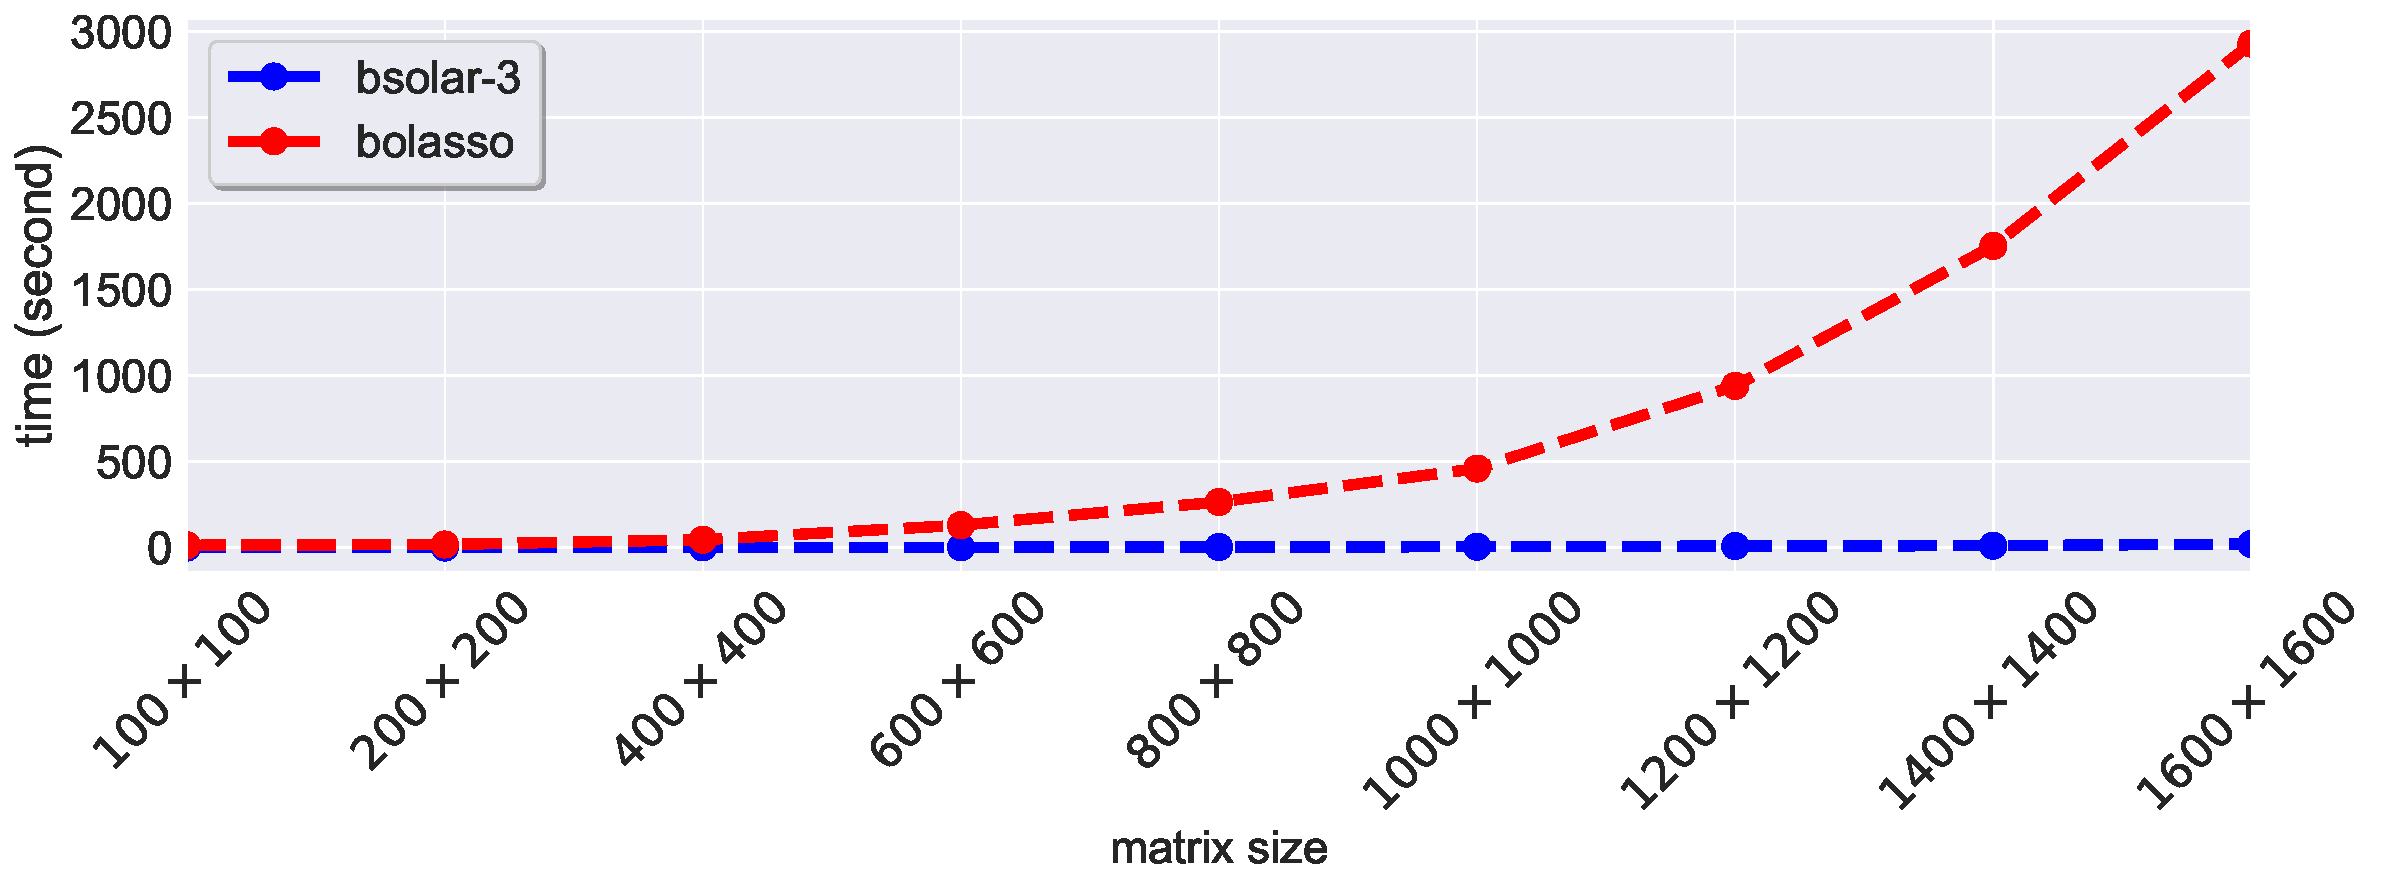
\includegraphics[width=0.8\linewidth]{runtime.pdf}
    %
    \caption{Average runtime (per pathwise coordinate descent) comparison for different $X$ matrix sizes.}
    %
    \label{fig:runtime}
    %
  \end{figure}
\end{frame}

\begin{frame}{Reference}
  \bibliographystyle{elsarticle-harv}
  \bibliography{ref/CVrefs}
\end{frame}

\end{document}
